\documentclass[aspectratio=169]{../latex_main/tntbeamer}  % you can pass all options of the beamer class, e.g., 'handout' or 'aspectratio=43'
\usepackage{dsfont}
\usepackage{bm}
\usepackage[english]{babel}
\usepackage[T1]{fontenc}
%\usepackage[utf8]{inputenc}
\usepackage{graphicx}
\graphicspath{ {./figures/} }
\usepackage{algorithm}
\usepackage[ruled,vlined,algo2e,linesnumbered]{algorithm2e}
\usepackage{hyperref}
\usepackage{booktabs}
\usepackage{mathtools}

\usepackage{amsmath,amssymb}

\DeclareMathOperator*{\argmax}{arg\,max}
\DeclareMathOperator*{\argmin}{arg\,min}

\usepackage{amsbsy}
\newcommand{\vect}[1]{\bm{#1}}
%\newcommand{\vect}[1]{\boldsymbol{#1}}

\usepackage{pgfplots}
\pgfplotsset{compat=1.16}
\usepackage{tikz}
\usetikzlibrary{trees} 
\usetikzlibrary{shapes.geometric}
\usetikzlibrary{positioning,shapes,shadows,arrows,calc,mindmap}
\usetikzlibrary{positioning,fadings,through}
\usetikzlibrary{decorations.pathreplacing}
\usetikzlibrary{intersections}
\pgfdeclarelayer{background}
\pgfdeclarelayer{foreground}
\pgfsetlayers{background,main,foreground}
\tikzstyle{activity}=[rectangle, draw=black, rounded corners, text centered, text width=8em]
\tikzstyle{data}=[rectangle, draw=black, text centered, text width=8em]
\tikzstyle{myarrow}=[->, thick, draw=black]

% Define the layers to draw the diagram
\pgfdeclarelayer{background}
\pgfdeclarelayer{foreground}
\pgfsetlayers{background,main,foreground}

% Requires XeLaTeX or LuaLaTeX
%\usepackage{unicode-math}

\usepackage{fontspec}
%\setsansfont{Arial}
\setsansfont{RotisSansSerifStd}[ 
Path=../latex_main/fonts/,
Extension = .otf,
UprightFont = *-Regular,  % or *-Light
BoldFont = *-ExtraBold,  % or *-Bold
ItalicFont = *-Italic
]
\setmonofont{Cascadia Mono}[
Scale=0.8
]

% scale factor adapted; mathrm font added (Benjamin Spitschan @TNT, 2021-06-01)
%\setmathfont[Scale=1.05]{Libertinus Math}
%\setmathrm[Scale=1.05]{Libertinus Math}

% other available math fonts are (not exhaustive)
% Latin Modern Math
% XITS Math
% Libertinus Math
% Asana Math
% Fira Math
% TeX Gyre Pagella Math
% TeX Gyre Bonum Math
% TeX Gyre Schola Math
% TeX Gyre Termes Math

% Literature References
\newcommand{\lit}[2]{\href{#2}{\footnotesize\color{black!60}[#1]}}

%%% Beamer Customization
%----------------------------------------------------------------------
% (Don't) Show sections in frame header. Options: 'sections', 'sections light', empty
\setbeamertemplate{headline}{empty}

% Add header logo for normal frames
\setheaderimage{
	% 
\includegraphics[height=\logoheight]{figures/TNT_darkv4.pdf}
	
\includegraphics[height=\logoheight]{../latex_main/figures/luh_logo_rgb_0_80_155.pdf}
	% 
\includegraphics[height=\logoheight]{figures/logo_tntluh.pdf}
}

% Header logo for title page
\settitleheaderimage{
	% 
\includegraphics[height=\logoheight]{figures/TNT_darkv4.pdf}
	
\includegraphics[height=\logoheight]{../latex_main/figures/luh_logo_rgb_0_80_155.pdf}
	% 
\includegraphics[height=\logoheight]{figures/logo_tntluh.pdf}
}

% Title page: tntdefault 
\setbeamertemplate{title page}[tntdefault]  % or luhstyle
% Add optional title image here
%\addtitlepageimagedefault{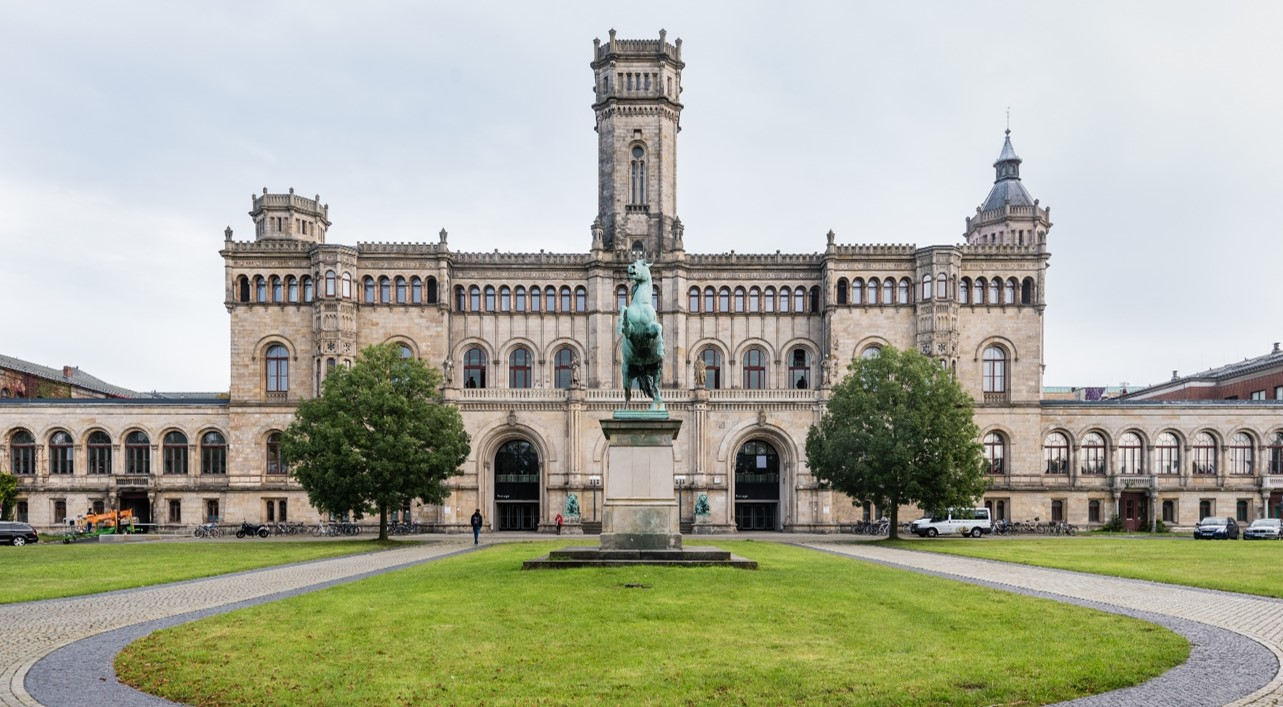
\includegraphics[width=0.65\textwidth]{figures/luh_default_presentation_title_image.jpg}}

% Title page: luhstyle
% \setbeamertemplate{title page}[luhstyle]
% % Add optional title image here
% \addtitlepageimage{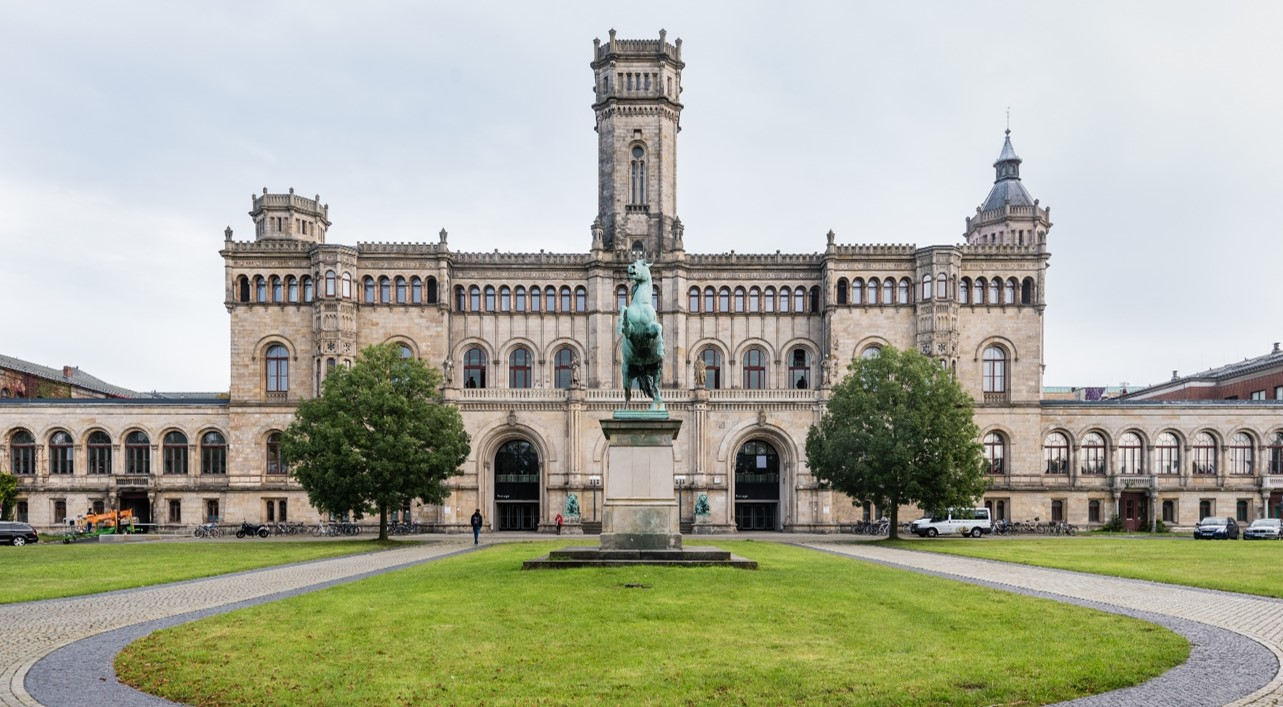
\includegraphics[width=0.75\textwidth]{figures/luh_default_presentation_title_image.jpg}}

\author[Abedjan \& Lindauer]{Ziawasch Abedjan \& Marius Lindauer\\[1em]
	
\includegraphics[height=\logoheight]{../latex_main/figures/luh_logo_rgb_0_80_155.pdf}\qquad
	
\includegraphics[height=\logoheight]{../latex_main/figures/DBIS_Kurzlogo.png}\qquad

\includegraphics[height=\logoheight]{../latex_main/figures/TNT_darkv4}\qquad

\includegraphics[height=\logoheight]{../latex_main/figures/L3S.jpg}	}
\date{Summer Term 2022; \hspace{0.5em} {
\includegraphics[height=1.5em]{../latex_main/figures/Cc-by-nc-sa_icon.svg.png}}; based on \href{https://ds100.org/fa21/}{[DS100]}
}


%%% Custom Packages
%----------------------------------------------------------------------
% Create dummy content
\usepackage{blindtext}

% Adds a frame with the current page layout. Just call \layout inside of a frame.
\usepackage{layout}


%%% Macros
%\renewcommand{\vec}[1]{\mathbf{#1}}
% \usepackage{bm}
%\let\vecb\bm

\title[Statistics]{DS: Bias and Variance}
\subtitle{Variance}

\graphicspath{ {./figure/} }
%\institute{}


\begin{document}
	
	\maketitle
	\begin{frame}{Definition of variance}
	    \begin{itemize}
	        \item \alert{Variance} is the expected squared deviation from the expectation of $X$.
	        \item It is defined as follows:
	        \begin{equation*}
	            \mathbb{V}ar(X) = \mathbb{E}\left[(X - \mathbb{E}(X))^2\right]
	        \end{equation*}
	        \item The units of the variance are the square of the units of $X$
	        \item To get back to the right scale, we look at the \alert{standard deviation} of $X$:
	        \begin{equation*}
	            \mathbb{SD}(X)  = \sqrt{\mathbb{V}ar(X)}  =\sqrt{\mathbb{E}((X - \mathbb{E}(X))^2)}
	        \end{equation*}
	        \item Both standard deviation and variance must be non-negative\\ because $x^2$ is non-negative for any $x$.
	    \end{itemize}
	\end{frame}
	
	
	\begin{frame}[c]{Interpretation of variance}
	    \begin{itemize}
	        \item The main use of variance is to quantify chance error.
	        \begin{itemize}
	            \item How far away from the expectation can $X$ be, just by chance?
	        \end{itemize}
	        \item By Chebyshev’s inequality:
	        \begin{itemize}
	            \item No matter what the shape of the distribution of $X$ is:
	            \item[$\leadsto$] The vast majority of the probability lies in the interval “expectation plus or minus a few standard deviations”.
	            \item Specifically, if   $\mu  = \mathbb{E}[X]$ and    $\sigma   = \mathbb{SD}[X]$, then $P(|X - \mu| \geq k\sigma) \leq \frac{1}{k^2}$.   
	        \end{itemize}
	    \end{itemize}
	\end{frame}
	
	
% 	\begin{frame}[c]{An alternative calculation}
% 	    There’s a more convenient form of variance for use in calculations.
% 	    \begin{equation*}
% 	        \mathbb{V}ar(X) = \mathbb{E}(X^2) - (\mathbb{E}(X))^2
% 	    \end{equation*}
% 	    To derive this, we make repeated use of the linearity of expectation.
% 	    \begin{align*}
% 	        \mathbb{V}ar(X) &= \mathbb{E}((X-\mathbb{E}(X))^2)\\
% 	        &=  \mathbb{E}(X^2-2X\mathbb{E}(X) + (\mathbb{E}(X)^2))\\
% 	        &= \mathbb{E}(X^2) - 2\mathbb{E}(X)\mathbb{E}(X) + (\mathbb{E}(X))^2\\
% 	        &= \mathbb{E}(X^2) - (\mathbb{E}(X))^2
% 	    \end{align*}
% 	\end{frame}
	
	
	
	\begin{frame}[c]{An alternative calculation}
	There’s a more convenient form of variance for use in calculations.
	    \begin{equation*}
	        \mathbb{V}ar(X) = \mathbb{E}(X^2) - (\mathbb{E}(X))^2
	    \end{equation*}
	    For example, to compute the variance of one roll of a die, we can find
	    \begin{equation*}
	        \mathbb{V}ar(X)= (1^2+2^2+3^2+4^2+5^2+6^2)\cdot \frac{1}{6}-(3.5)^2 = 2.92
	    \end{equation*}
	    
	    \begin{itemize}
	        \item This formulation also makes clear that if X is centered, i.e. $\mathbb{E}(X) = 0$, then $\mathbb{V}ar(X) = \mathbb{E}(X^2)$.
	        \item Since $\mathbb{V}ar(X)$ is non-negative, this property also shows us that $\mathbb{E}(X^2) \geq (\mathbb{E}(X))^2$.
	        \item Equality is if and only if $X$ is a constant.
	        \item If you know the expectation and variance of a random variable, you can easily determine the expectation of its square:   $\mathbb{E}(X^2) = \mathbb{V}ar(X) + (\mathbb{E}(X))^2$. 
	    \end{itemize}
	\end{frame}
	
	
	\begin{frame}[c]{Linear transformations}
	    
	    \begin{itemize}
	        \item We know that  $\mathbb{E}(aX + b) = a\mathbb{E}(X) + b$.
	        \item In order to compute $\mathbb{V}ar(aX + b)$, consider:\\
	    \end{itemize}
	    
	    \begin{columns}
	    
	        \begin{column}{.5\textwidth}
	        
	                A shift by $b$ units does not affect spread:

                        \centering
	                    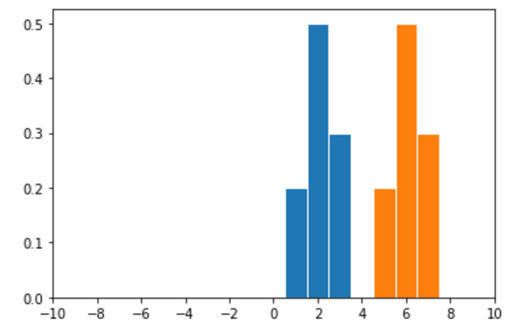
\includegraphics[scale=.5]{Bild7}
	                    
	                Here, the distribution of $X$ is in blue, and the distribution of $X+4$ is in orange.
	        \end{column}
	        
	        
	        \begin{column}{.5\textwidth}
	        
	                But scaling by a units does affect spread:
                        
                        \centering
	                    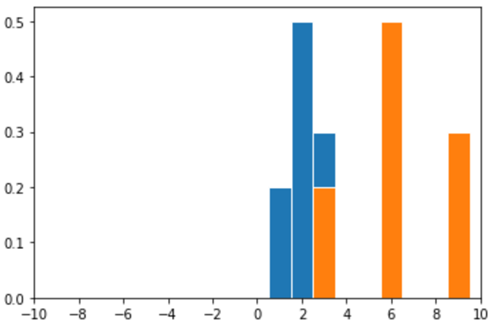
\includegraphics[scale=.35]{Bild8}

	                The distribution of $X$ is in blue, and the distribution of $3X$ is in orange. 
	        \end{column}
	    \end{columns}
	\end{frame}
	
	
	\begin{frame}[c]{Linear transformations}
	   We know that $\mathbb{E}(aX + b) = a\mathbb{E}(X) + b$. \\                  
	   In order to compute $\mathbb{V}ar(aX + b)$, consider:
	    \begin{itemize}
	        \item A shift by $b$ units does not affect spread. Thus, $\mathbb{V}ar(aX + b) = \mathbb{V}ar(aX)$.
	        \item The multiplication by a does affect spread!
	    \end{itemize}
	    Then,
	    \begin{align*}
	        \mathbb{V}ar(aX + b) = \mathbb{V}ar(aX) &= \mathbb{E}((aX)^2) - (\mathbb{E}(aX))^2\\
	        &= \mathbb{E}(a^2X^2) - (a\mathbb{E}(X))^2\\
	        &= a^2(\mathbb{E}(X^2) - (\mathbb{E}(X))^2)\\
	        &= a^2\mathbb{V}ar(X)
	    \end{align*}
	    In summary:
	    \begin{align*}
	        \mathbb{V}ar(aX + b) &= a^2\mathbb{V}ar(X)\\
	        \mathbb{SD}(aX + b) &= |a|\mathbb{SD}(X)
	    \end{align*}
	\end{frame}
	
	
	\begin{frame}[c]{Standardization of random variables}
	   $X$ in standard units is the random variable $X_{su} = \frac{X- \mathbb{E}(X)}{\mathbb{SD}(X)}$
	   \begin{itemize}
	       \item $X_{su}$ measures X on the scale “number of SDs from expectation.”
	       \item It is a linear transformation of X. By the linear transformation rules for expectation and variance:
	       \begin{equation*}
	           \mathbb{E}(X_{su})  = 0, \hspace{5mm} \mathbb{SD}(X_{su}) = 1
	       \end{equation*}
	       \item Since $X_{su}$ is centered (has expectation 0):
	       \begin{equation*}
	           \mathbb{E}(X^2_{su}) = \mathbb{V}ar(X_{su}) = 1
	       \end{equation*}
	       
	       \item \alert{Note}: Standardization of your data with $\mu$ and $\sigma$ makes most sense\\ if your data is Gaussian distributed
	       \begin{itemize}
	           \item Don't blindly apply data transformations! 
	       \end{itemize}
	       
	   \end{itemize}
	\end{frame}
	
	\begin{frame}[c]{Covariance}
	   The covariance of two random variables is their expected product of deviations.
	   \begin{equation*}
	       \mathbb{C}ov(X,Y) = \mathbb{E}((X-\mathbb{E}(X))(Y-\mathbb{E}(Y)))
	   \end{equation*}
	   \begin{itemize}
	       \item It is a generalization of variance. 
	       \item Note: $\mathbb{C}ov(X,X) = \mathbb{V}ar(X)$.   
	       \item Using the linearity of expectation and some algebra, you can show the following equality, which is a generalization of the alternative calculation for variance:
	       \begin{equation*}
	           \mathbb{C}ov(X,Y) = \mathbb{E}(XY) - \mathbb{E}(X)\mathbb{E}(Y)
	       \end{equation*}
	       \item To see whether variance is ever additive, we need to look at covariance differently.
	   \end{itemize}
	\end{frame}
	
	\begin{frame}[c]{Correlation}
	   The units of the covariance are hard to interpret because they ``mix'' two RVs.
	   
	   In order to get rid of the units, we can scale it:
	   
	   \begin{align*}
	       \frac{\mathbb{C}ov(X,Y)}{\mathbb{SD}(X)\mathbb{SD}(Y)}  &= \frac{ \mathbb{E}((X-\mathbb{E}(X))(Y-\mathbb{E}(Y)))}{\mathbb{SD}(X)\mathbb{SD}(Y)}\\
	       &= \mathbb{E}\left( \frac{X-\mathbb{E}(X)}{\mathbb{SD}(X)} \cdot \frac{Y-\mathbb{E}(Y)}{\mathbb{SD}(Y)}\right)\\
	       &= \mathbb{E}(X_{su}Y_{su})\\
	       &= r(X,Y)
	   \end{align*}
	   \alert{Correlation is covariance scaled by the two SDs!}
	\end{frame}
\end{document}